\begin{tcolorbox}[colback=white,colframe=black,opacityframe=0,colbacktitle=black,title={\textbf{Problem 2 [\examproblemweight\ points]}}]
Consider the following relations, either defined as a graph or as an equation. For each of these:
\begin{enumerate}[label=(\roman*)]
	\item Is this a function? If it is, you do not have to explain why. If it is \emph{not}, explain why.
	\item If this is a function, is this one-to-one? \emph{You must explain why if it is one-to-one, or if it is not.} (If this relation was not a function in the first place, you do not need to answer this part.)
\end{enumerate}
\begin{enumerate}[label=(\alph*)]
	\item 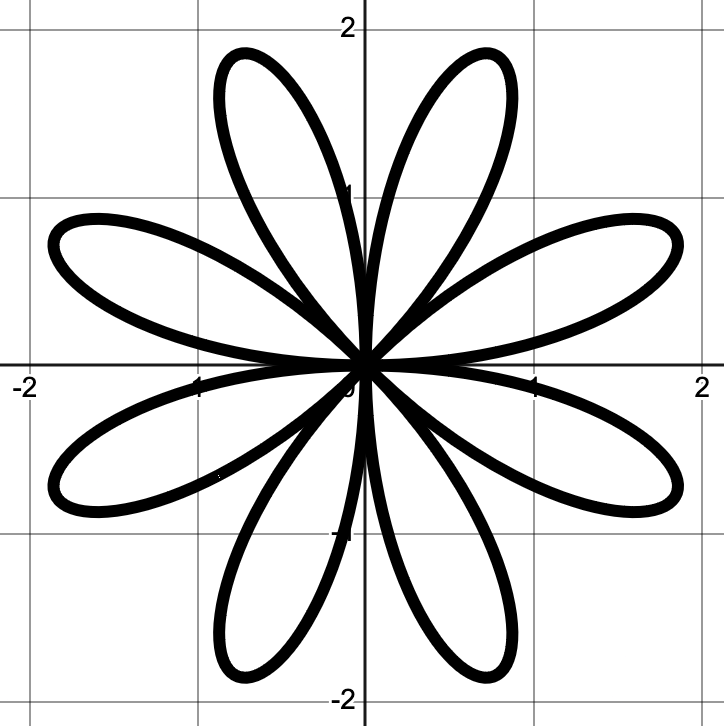
\includegraphics[scale=0.15]{midterm/2_1.png}  \hspace*{10em}
	\inlineitem 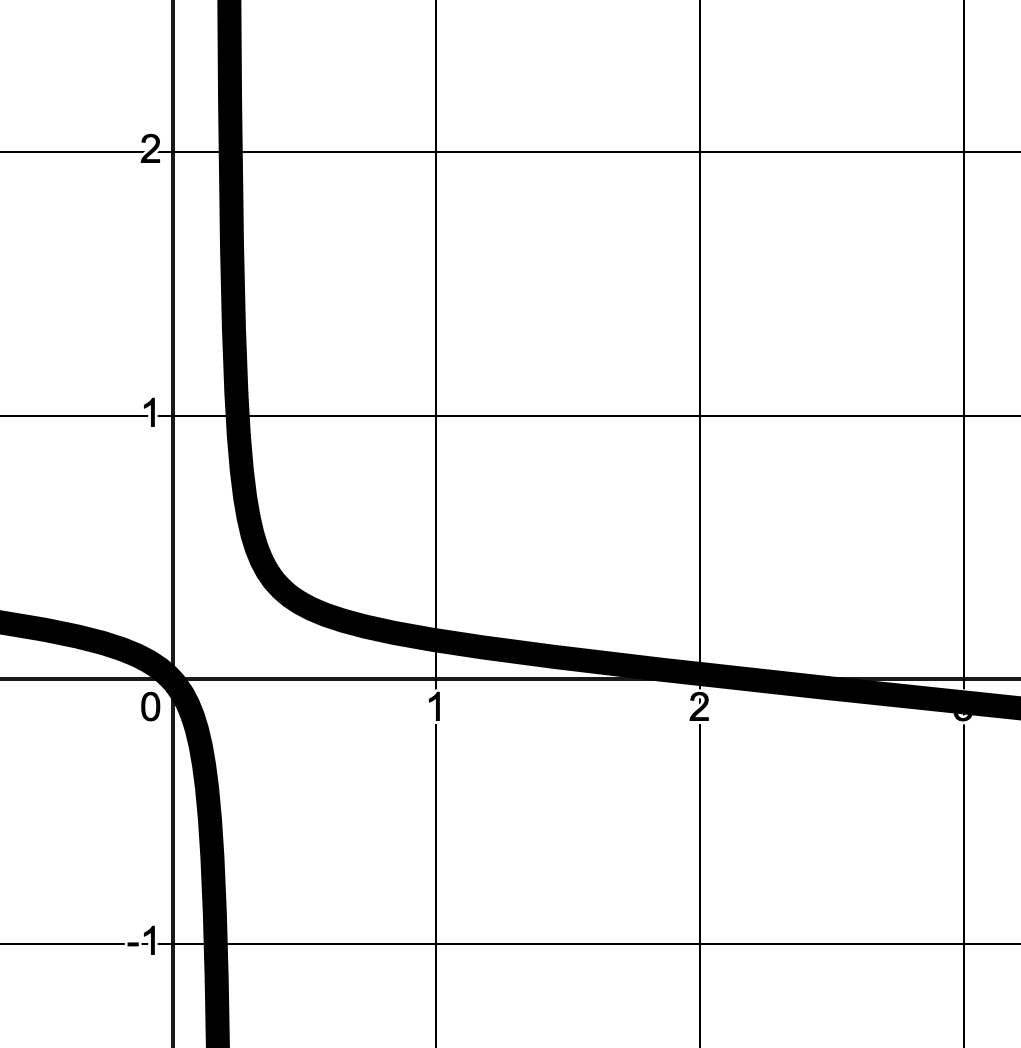
\includegraphics[scale=0.1]{midterm/2_2.png}
	\vspace*{8em}
	\item $|x+4|+y=-1$ \hspace*{13.5em}
	\inlineitem $x^2 + (y-2)^2 = 1$
\end{enumerate}

\end{tcolorbox}

\newpage
\noindent \centering Blank page \thepage~for additional work
\newpage